\documentclass[12pt]{article}
\usepackage[utf8]{inputenc}
\usepackage[english]{babel}
\usepackage{amsmath,amssymb,amsfonts}
\usepackage{xcolor}
\usepackage{graphicx}
\usepackage{caption}
\usepackage{subcaption}
\usepackage{hyperref}
\usepackage{float}
\usepackage{multicol}
\usepackage{blindtext}
\usepackage{geometry}
\geometry{
	a4paper,
	total={190mm,267mm}, % a4 is 210 x 297 mm
	left=10mm,
	top=17mm,
}

%code
\usepackage{listings}
\definecolor{codegreen}{rgb}{0,0.6,0}
\definecolor{codegray}{rgb}{0.5,0.5,0.5}
\definecolor{codepurple}{rgb}{0.58,0,0.82}
\definecolor{backcolour}{rgb}{0.95,0.95,0.92}

\lstdefinestyle{mystyle}{
	backgroundcolor=\color{backcolour},   
	commentstyle=\color{codegreen},
	keywordstyle=\color{magenta},
	numberstyle=\tiny\color{codegray},
	stringstyle=\color{codepurple},
	basicstyle=\ttfamily\footnotesize,
	breakatwhitespace=false,         
	breaklines=true,                 
	captionpos=b,                    
	keepspaces=true,                 
	numbers=left,                    
	numbersep=5pt,                  
	showspaces=false,                
	showstringspaces=false,
	showtabs=false,                  
	tabsize=2
}

\lstset{style=mystyle}

\usepackage{tabularx}
%\lstset{ 
%	upquote=true,
%	columns=fullflexible,
%	basicstyle=\ttfamily,
%	literate={*}{{\char42}}1
%	{-}{{\char45}}1
%	{\ }{{\copyablespace}}1
%}

\usepackage{algorithm}
\usepackage{algpseudocode}

\usepackage[space=true]{accsupp}
\newcommand{\copyablespace}{\BeginAccSupp{method=hex,unicode,ActualText=00A0}\hphantom{x}\EndAccSupp{}}
\title{\sffamily The Mutually Orthogonal Legendre Polynomials }
\author{\sffamily Shashvat Jain\\ \sffamily (2020PHY1114)(20068567054)}
\begin{document}

%\begin{abstract}

%\end{abstract}
\begin{titlepage}
	\renewcommand\familydefault{\sfdefault}
	\fontfamily{stix}\selectfont
	\maketitle
	\vspace{4cm}
	\begin{center}
		\large Lab Report for Assignment No. 2b
	\end{center}
	\vspace{4cm}

	\begin{table}[h]
		\centering	
		\begin{tabularx}{0.55\textwidth}{lr}		
			College Roll No :& 2020PHY1114\\
			University Roll NoName:& 20068567054\\
			Unique Paper Code: &32221401\\
			Paper Title: &Mathematical physics III Lab\\
			Course and Semester :&B.Sc.(H) Physics Sem IV\\
			Due Date: & Jan 15,2022\\
			Date of Submission:& Jan 14,2022\\
			Lab Report File Name:& mp3A2b\_2020PHY1114.pdf\\
			Partner’s Name:& -\\
			Partner’s College  Roll No.:& \sffamily -\\
		\end{tabularx}
	\end{table}
	
	\pagenumbering{gobble}
\end{titlepage}
\newpage
\pagenumbering{arabic}
\section{Theory}
Polynomials or Polynomial functions $ P_1(x):\mathbb{R}\rightarrow  \mathbb{R} $ and $ P_2(x) : \mathbb{R} \rightarrow \mathbb{R}$ are called \textbf{orthogonal} in the closed interval $ [a,b] $ if and only if $ {\displaystyle \int_{a}^{b}P_1 P_2 dx } = 0 $. The idea is analogous to the orthogonality of finite-dimensional vectors where we define orthogonality of two vectors by a null valued dot product. Since a polynomial function is a real-valued mapping into $ \mathbb{R} $ it is a part of the vector space of all functions from $ \mathbb{R} \rightarrow \mathbb{R} $. We define an operation called the standard \textbf{inner-product} just like the dot-product which when found to be zero declares the orthogonality of the constituent elements of the space.\\[2mm]
The Orthogonality condition for Legendre polynomials $ P_k $ where $ k $ give the order of the polynomial is given by,
\begin{equation} \label{ortho-leg:}
	{\displaystyle \int _{-1}^{1}P_{m}(x)P_{n}(x)\,dx=\left\{\begin{array}{lr}
			\frac{2}{2n+1} & \text{ for } m=n\\
			0 & \text{ for } m\neq n 
		\end{array}\right\}={\frac {2}{2n+1}}\delta _{mn},}
\end{equation}
\noindent \\
Given starting basis of linearly independent functions $ B = \{1,x,x^2,x^3,x^4,\dots \} $, let us take the constant polynomial function $L_0(x) = 1 $ to be the first element in the newly made basis  $ L $ orthogonal in the interval $ \left[-1,1 \right] $.
Now, 
\begin{align}
	L_1 &= x - \frac{<x,1>}{<1,1>}1 \nonumber\\
	&= x - \frac{\int_{-1}^{1}xdx}{\int_{-1}^{1}dx} = x  \\
	L_2 &= x^2 - \frac{<x,x^2>}{<x,x>}x - \frac{<x^2,1>}{<1,1>}1 \nonumber \\
	&= x^2 - \frac{\int_{-1}^{1}x^3dx}{\int_{-1}^{1}x^2dx}x - \frac{\int_{-1}^{1}x^2dx}{\int_{-1}^{1}dx} = x^2 - \frac{1}{3} 
\end{align}
Therefore $ L = \{1,x,x^2-1/3\} $. Now since $\frac{2}{3}L_3$ is a scaled version of $ L_3 $ it also is orthogonal to all other elements of $ L $, 
the orthogonal basis $ { L' = \left\{1,x,\frac{1}{2}(3x^2 - 1)\right\}}$ have all its elements as solutions to the Legendre differential equation.\\

\noindent
By Definition,
\begin{equation}
	f(x) = \sum_{n=0}^{\infty}C_n P_n(x)
\end{equation}
To find a coefficient $ C_k $ Multiplying both sides by $ P_k $ and integrating both sides with respect to $ x $ from -1 to 1.
\begin{align}
	\int_{-1}^{1}P_k(x)f(x)dx &= \int_{-1}^{1}P_k\sum_{n=0}^{\infty}  C_n P_n dx \nonumber \\
	\implies \int_{-1}^{1}P_k(x)f(x)dx &= \sum_{n=0}^{\infty} \int_{-1}^{1}P_k(x)  C_n P_n(x) dx \nonumber \\
	\implies \int_{-1}^{1}P_k(x)f(x)dx &= \sum_{n=0}^{\infty} \int_{-1}^{1}P_k(x)  C_n P_n(x) dx \nonumber \\
	\implies \int_{-1}^{1}P_k(x)f(x)dx &= \int_{-1}^{1}C_0P_k(x)P_0(x) dx+\int_{-1}^{1}C_1P_k(x)P_1(x) dx + \dots +\int_{-1}^{1}C_kP_k(x)P_k(x) dx +\dots \nonumber
\end{align}
From \ref{ortho-leg:} all terms except one with $n=k$ go to zero, leaving behind,
\\
\begin{align} \label{coef}
	&\int_{-1}^{1}P_k(x)f(x)dx =C_k \frac{2}{2k+1} \nonumber \\ 
	&\boxed{C_k = \frac{2k +1}{2} \int_{-1}^{1}P_k(x)f(x)dx }
\end{align}
\noindent \\
Since all Legendre polynomials are orthogonal to each other, The set of all Legendre polynomials of order less than equal to $ n \in N $, since they are linearlty independent, span the function space of all polynomials of order less than equal to $ n $. Therefore the series expansion of any polynomial function of order $ n $ will have atmost $n(\{P_n,P_{n-1},P_{n-2}\dots P_0\})  = n+1$ terms.\\ 
\noindent \\
($\alpha$)Using the above relation \ref{coef} we can deduce the coefficients which come out to be:\\

\begin{multicols}{2}
\begin{align*}
	C_0 &= \frac{1}{2}\int_{-1}^{1}(1)(2+3x+2x^4)dx
\\
	&=\frac{1}{2}\left(\frac{24}{5}\right)
\\
	&=\frac{12}{5}
\end{align*}
\begin{align*}
	C_1&=\frac{3}{2}\int_{-1}^{1}(x)(2+3x+2x^4)dx
\\
	&=\frac{3}{2}(2) \\
	&=3
\end{align*}

\begin{align*}
	C_2&=\frac{5}{2}\int_{-1}^{1}\frac{1}{2}(3x^2-1)(2+3x+2x^4)dx\\&=\frac{5}{2}\left(\frac{16}{35}\right)\\&= \frac{8}{7}
\end{align*}
\begin{align*}
	C_3&=\frac{7}{2}\int_{-1}^{1}\frac{1}{2}(5x^3-3x)(2+3x+2x^4)dx\\&=\frac{7}{2}(0)=0	
\end{align*}
\begin{align*}
	C_4&=\frac{9}{2}\int_{-1}^{1}\frac{1}{8}(35x^4-30x^2+3)(2+3x+2x^4)dx
\\
	&=\frac{9}{2}\left(\frac{32}{315}\right)
\\
	&=\frac{16}{35}
\end{align*}
\end{multicols}
$\displaystyle f(x)=\left(\frac{12}{5}\right) P_0+(3)P_1+\left(\frac{8}{7}\right)P_2+(0)P_3+\left(\frac{16}{35}\right)P_4$
\\
($\beta$) We have to find the first 5 terms of the expansion so,
\begin{multicols}{2}
\begin{align*}
	C_0 &= \frac{1}{2}\int_{-1}^{1}(1)(\cos(x)\sin(x))dx
\\
	&=\frac{1}{2}(0)
\\
	&=0
\end{align*}
\begin{align*}
	C_1&=\frac{3}{2}\int_{-1}^{1}(x)(\cos(x)\sin(x))dx
\\
	&=\frac{3}{2}(0.43540)
\\
	&=0.6531
\end{align*}
\end{multicols}
\begin{multicols}{2}
\begin{align*}
	C_2&=\frac{5}{2}\int_{-1}^{1}\frac{1}{2}(3x^2-1)(cos(x)sin(x))dx
\\
	&=\frac{5}{2}(0)
\\
	&= 0
\end{align*}

\begin{align*}
	C_3&=\frac{7}{2}\int_{-1}^{1}\frac{1}{2}(5x^3-3x)(cos(x)sin(x))dx
\\
	&=\frac{7}{2}(-0.060722)
\\
	&= -0.212527
\end{align*}

\begin{align*}
	C_4&=\frac{9}{2}\int_{-1}^{1}\frac{1}{8}(35x^4-30x^2+3)(cos(x)sin(x))dx
\\
	&=\frac{9}{2}(0)
\\
	&= 0
\end{align*}

\end{multicols}
$f(x)=(0)P_0+(0.6531)P_1+(0)P_2+(-0.212527)P_3+(0)P_4$\\
\section{Analysis}

\textbf{NOTE: $f_n$ is the notation used for the Legendre series approximate of f calculated upto first n terms or the n-th partial sum of the series $ \sum_{n=0}^{\infty} C_n P_n $}
\\
\noindent \\
For problem 2(a):\\
The first array in figure represents the non-zero coefficients of the series corresponding to the order of polynomials in the second array.
$[2.4        3.         1.14285714 0.45714286] [0 1 2 4]$
i.e. $C_0 = 2.4 , C_1 = 3 , C_2 = 1.14285714$

\noindent \\
For problem 2(b):\\
Max difference between values of $f_2-f_1$: 2.0517636768997254 \\
RMS ERROR between values of $f_2-f_1$: 0.17091050427990304 \\ 
Max difference between values of $f_3-f_2$: 4.440892098500626e-16 \\
RMS ERROR between values of $f_3-f_2$: 2.9123522237328004e-17 \\
Accuracy of 6 significant digits reached with number of terms equal to: 2 \\

\begin{figure}[H]
	\centering
	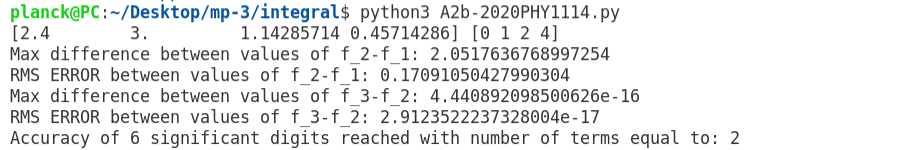
\includegraphics[width=\linewidth]{part2_output.png}
\end{figure}

\noindent \\
From the first subplot for $f(x) = 2 x^4 + 3x + 2$ we can clearly see that $f_5$ overlaps the graph of the true values of f, hence representing the function $f$ exactly, verified using zero RMSE in the domain for 50 nodes where the series was calculated.
Therefore we verified that a polynomial of order $k$ can be represented exactly as a weighted sum of Legendre polynomials of order $\leq k$ (k+1 terms.)
\\
\noindent 
From the second plot for $ f(x) = \sin(x)\cos(x) $ we see that since the function is not a polynomial function, the approximation of f using legendre polynomials upto first 8 terms produces a very small error and 10 terms produce even smaller values of RMS, this trend is justified as it is in agreement with the priori that f is exactly represented by the weighted sum of Legendre polynomials as no. of terms go to infinity.
\\

\begin{figure}[H]
	\centering
	\def\svgwidth{\columnwidth}
	\input{function_plots.pdf_tex}
	\caption{Functions obtained as a linear combination of Legendre polynomials plotted in the range $[-2,2]$ for different number of terms.}
\end{figure}

\section{Appendix}

\subsection{Code}

\lstinputlisting[language= Python]{/home/planck/Desktop/mp-3/integral/fourier_legendre.py}
\lstinputlisting[language=Python]{/home/planck/Desktop/mp-3/integral/A2b-2020PHY1114.py}

\end{document}
